\section{Liquid-Chromatography}

\frame[noframenumbering]{
    \frametitle{Liquid-Chromatography principle}
    
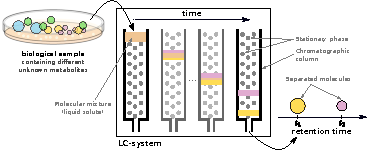
\includegraphics[width=\textwidth]{images/lc_concept.pdf}
}

\section{Molecular fingerprints}

\frame[noframenumbering]{
%     \frametitle{Compare binary and counting molecular fingerprints}
    \frametitle{Molecules represented using MACCS dictionary fingerprints}

\begin{figure}
    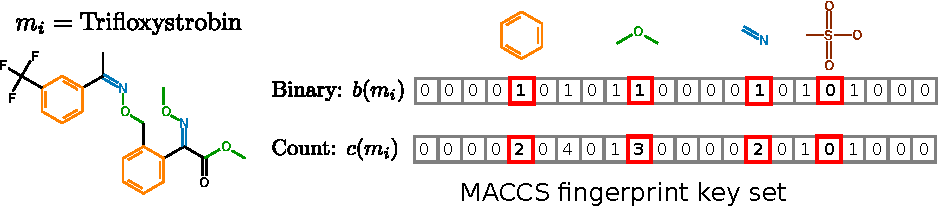
\includegraphics[width=\textwidth]{images/fingerprint_example.pdf}
\end{figure}
\begin{block}{Kernels used for the feature embedding in RankSVM}
\vspace{-0.25cm}
% \begin{small}
\begin{itemize}
    \item Binary: Tanimoto kernel \cite{Ralaivola2005}
\begin{center}
    $\kmol(m_i,m_j)=\frac{|b(m_i)\cap b(m_j)|}{|b(m_i)\cup b(m_j)|}$%\frac{b(m_i)^T b(m_j)}{b(m_i)^T b(m_i)+b(m_j)^T b(m_j)-b(m_i)^T b(m_j)}$
\end{center}
    \item Count: MinMax kernel \cite{Ralaivola2005}
\begin{center}
    $\kmol(m_i,m_j)=\frac{\sum_{s=1}^{N_{sub}}\min(c_s(m_i),c_s(m_j))}{\sum_{s=1}^{N_{sub}}\max(c_s(m_i),c_s(m_j))}$
\end{center}
\end{itemize}
% \end{small}
\end{block}
}

\frame[noframenumbering]{ 
    \frametitle{Compare binary and counting molecular fingerprints}
%     \framesubtitle{Encoding molecular structures using MACCS dictionary molecular fingerprints.}

\begin{itemize}
    \item Pairwise prediction accuracy ($\pm 2\sigma$) for different target systems
    \item RankSVM models trained using single system $\Pref(\sys)$.
\end{itemize}

\begin{table}[!t]
\begin{tabular}{@{}lcc@{}}
    \toprule 
    Target system $\sys$ & Binary MACCS & Counting MACCS \\\midrule
    Eawag\_XBridgeC18 & $0.796 (\pm 0.015)$ & $\mathbf{0.844 (\pm 0.011)}$ \\
    FEM\_long         & $0.882 (\pm 0.016)$ & $\mathbf{0.905 (\pm 0.015)}$ \\
    RIKEN             & $0.826 (\pm 0.024)$ & $\mathbf{0.848 (\pm 0.017)}$ \\
    UFZ\_Phenomenex   & $0.790 (\pm 0.027)$ & $\mathbf{0.802 (\pm 0.017)}$ \\
    LIFE\_old         & $0.842 (\pm 0.050)$ & $\mathbf{0.862 (\pm 0.035)}$ \\
    \bottomrule
\end{tabular}
\end{table} 
}
